% Sablon pentru realizarea lucrarii de licenta, conform cu recomandarile
% din ghidul de redactare:
% - https://fmi.unibuc.ro/finalizare-studii/

% Multumiri lui Gabriel Majeri, acest sablon a fost creat pe baza
% codului sursa a lucrarii sale de licenta. 
% Codul sursa: https://github.com/GabrielMajeri/bachelors-thesis
% Website: https://www.gabrielmajeri.ro/
%
% Acest sablon este licentiat sub Creative Commons Attribution 4.0 International License.
% modificat 8 noiembrie 2024

\documentclass[12pt, a4paper]{report}

% Font Times New Roman
\usepackage{times}

% Suport pentru diferite stiluri de ghilimele
\usepackage{csquotes}

% Utilizează biblatex pentru referințe bibliografice
\usepackage[
    maxbibnames=50,
    sorting=nty
]{biblatex}

\addbibresource{bibliography.bib}

% Setează spațiere inter-linie (doublespacing din LaTeX este echivalentul setarii 1.5 in Microsoft Word)
\usepackage{setspace}
\doublespacing

% Modificarea geometriei paginii (cu margini de 2,5 cm) 
\usepackage[margin=2.5cm]{geometry}

% Include funcțiile de grafică
\usepackage{graphicx}
% Încarcă imaginile din directorul `images`
\graphicspath{{./images/}}

% Listări de cod
\usepackage{listings}

% Linkuri interactive în PDF
\usepackage[
    colorlinks,
    linkcolor={black},
    menucolor={black},
    citecolor={black},
    urlcolor={blue}
]{hyperref}

% Comenzi matematice
\usepackage{amsmath}
\usepackage{mathtools}

\usepackage{amssymb}

% Formule matematice
\newcommand{\bigO}{\mathcal{O}}
\DeclarePairedDelimiter\abs{\lvert}{\rvert}
\newcommand{\GF}[1]{$\text{GF}(2^{#1})$}
\newcommand{\bitand}{\;\&\;}

\newenvironment{abstractpage}
  {\cleardoublepage\vspace*{\fill}\thispagestyle{empty}}
  {\vfill\cleardoublepage}
\renewenvironment{abstract}[1]
  {\bigskip
   \begin{center}\bfseries\abstractname\end{center}}
  {\par\bigskip}
\newenvironment{rezumat}[1]
  {\bigskip
   \begin{center}\bfseries Rezumat \end{center}}
  {\par\bigskip}

% Suport pentru anexe
\usepackage{appendix}

% Stiluri diferite de headere și footere
\usepackage{fancyhdr}

\usepackage{indentfirst}

\usepackage{algorithm}
\usepackage{algpseudocode}

\usepackage{subcaption}

\usepackage{enumitem}

% Metadate
\title{File Corruption Repair \\Using Reed-Solomon Codes}
\author{Theodor Negrescu}

% Generează variabilele cu @
\makeatletter

\begin{document}

% Front matter
\cleardoublepage
\let\ps@plain

% Pagina de titlu
\begin{titlepage}

% Redu marginile
\newgeometry{left=2cm,right=2cm,bottom=1cm}

\begin{figure}[!htb]
    \centering
    \begin{minipage}{0.2\textwidth}
        
\includegraphics[width=\linewidth]{logo-ub.png}
    \end{minipage}
    \begin{minipage}{0.5\textwidth}
        \large
        \vspace{0.2cm}
        \begin{center}
            \textbf{UNIVERSITATEA DIN BUCUREȘTI}
        \end{center}
        \vspace{0.3cm}
        \begin{center}
            \textbf{
                FACULTATEA DE \\
                MATEMATICĂ ȘI INFORMATICĂ
            }
        \end{center}
    \end{minipage}
    \begin{minipage}{0.2\textwidth}
        
\includegraphics[width=\linewidth]{logo-fmi.png}
    \end{minipage}
\end{figure}

\begin{center}
\textbf{SPECIALIZAREA INFORMATICĂ}
\end{center}

\vspace{1cm}

\begin{center}
\Large \textbf{Project Report}
\end{center}

\begin{center}
\huge \textbf{\MakeUppercase{\@title}}
\end{center}

\vspace{3cm}

\begin{center}
\large \textbf{\@author}
\end{center}

\vspace{0.25cm}

\begin{center}
\large \textbf{Coordonator științific \\ Cristian Rusu}
\end{center}

\vspace{2cm}

\begin{center}
\Large \textbf{București, ianuarie 2025}
\end{center}
\end{titlepage}
\restoregeometry
\newgeometry{
    margin=2.5cm
}

\fancypagestyle{main}{
  \fancyhf{}
  \renewcommand\headrulewidth{0pt}
  \fancyhead[C]{}
  \fancyfoot[C]{\thepage}
}

\addtocounter{page}{1}

% Rezumatul
\begin{abstractpage}

\begin{abstract}


The aim of this project is to implement file corruption detection and repair using Reed-Solomon error-correcting codes.

The code used is an erasure code over the field \GF{64}, implemented using $O(n \log n)$ transforms in a polynomial basis introduced by Sian-Jheng Lin, Wei-Ho Chung, and Yunghsiang S. Han in \cite{novel-poly}.

Finite field multiplication is implemented using carry-less multiplication, also known as XOR multiplication, and division is implemented using the extended Euclidean algorithm.

The implementation is a command-line utility which can generate parity data for a file, and later detect and repair corruption in that file.

The file is split into $N$ blocks, and an arbitrary number of parity blocks $M$ can be generated, for a total of $N + M$ blocks.
Any $N$ blocks are sufficient to recover the original data, so up to $M$ corrupted blocks can be repaired.

As erasure codes require known error locations - the term 'erasure' refers to an error at a known location - a hash of each block is stored in the file header to detect corruption.

The file is not a single Reed-Solomon code, as that would require reading the entire file into memory, limiting the maximum file size which can be processed.
Instead, the file is interpreted as a matrix with $N + M$ rows, and each column is a separate Reed-Solomon code.

\vspace*{\fill}
\begin{center}Source code available at \url{https://github.com/theo543/rsarc}\end{center}

\end{abstract}

\end{abstractpage}

\begin{abstractpage}

\begin{rezumat}

\indent

Acest proiect are ca scop implementarea detecției și reparării coruperii fișierelor folosind coduri Reed-Solomon de corectare a erorilor.

Codul folosit este un cod de ștergere peste corpul \GF{64}, implementat folosind transformări în timp $O(n \log n)$ într-o bază polinomială introdusă de Sian-Jheng Lin, Wei-Ho Chung, și Yunghsiang S. Han în \cite{novel-poly}.

Înmulțirea în corp finit este implementată folosind înmulțire fără retenție ('carry-less'), uneori cunoscută ca înmulțire XOR, iar împărțirea este implementată folosind algoritmul extins al lui Euclid.

Implementarea este un utilitar de linie de comandă care poate genera date de paritate pentru un fișier și, ulterior, să detecteze și repare corupție în fișier.

Fișierul este împărțit în $N$ blocuri, și un număr arbitrar de blocuri de paritate $M$ pot fi generate, pentru un total de $N + M$ blocuri.
Orice $N$ blocuri sunt suficiente pentru a recupera datele originale, deci cel mult $M$ blocuri corupte pot fi reparate.

Deoarece un cod de ștergere necesită cunoașterea locațiilor erorilor - termenul 'ștergere' înseamnă o eroare la o locație cunoscută - un hash al fiecărui bloc este stocat în antetul fișierului pentru a detecta corupție.

Fișierul nu este un singur cod Reed-Solomon, deoarece ar necesita citirea întregului fișier în memorie, limitând dimensiunea maximă de fișier care poate fi procesată.
De fapt, fișierul este interpretat ca o matrice cu $N + M$ rânduri, iar fiecare coloană este un cod separat Reed-Solomon.

\vspace*{\fill}
\begin{center}Cod sursă disponibil la \url{https://github.com/theo543/rsarc}\end{center}

\end{rezumat}

\end{abstractpage}


\tableofcontents

% Main matter
\cleardoublepage
\pagestyle{main}
\let\ps@plain\ps@main

\chapter{Introduction}

Data corruption is a significant issue in software and hardware systems, which can lead to data loss, incorrect program behavior, and system failures.

It is impossible in general to prevent errors due to uncontrolled factors such as electromagnetic interference, cosmic rays, or hardware defects, not to mention software bugs.
Even data stored in memory or in CPU registers and cache will rarely be randomly corrupted, which must be accounted for in massive systems where it is statistically likely that regular errors will occur.

While in some cases only error detection is required, such as for network protocols which can resend data, in other cases full error correction is necessary, such as in cloud storage, backups, ECC RAM, RAID systems, and more.

Error detection and correction is a major area of research in the field of computer science, and many companies invest heavily in ensuring the robustness of their systems against random errors:

\begin{itemize}
    \item Major cloud storage providers guarantee that data is stored redundantly and split across multiple locations, and that is it regularly scanned for errors.
    \item Server hardware often includes ECC memory, which can transparently correct certain errors in RAM, and which will crash the system instead of silently saving corrupted data when it cannot be corrected.
    \item Modern filesystems such as ZFS and Btrfs automatically detect block-level errors using checksums, and have built-in support for redundancy.
    \item RAID technology (Redundant Array of Independent Disks) can combine multiple disk drives into one logical unit, and store data redundantly such that a disk failure causes no data loss,
          with various configurations allowing for different tradeoffs between storage capacity and redundancy.
\end{itemize}

While merely detecting errors with checksums or hashes is easy, being able to correct them without having full copies of the data is a complex task that requires error-correcting codes (ECC).

A major family of error-correcting codes is Reed-Solomon codes, which have a wide range of applications, such as in CDs, DVDs, radio transmissions, QR codes, and more.
Some configurations of RAID arrays use Reed-Solomon codes to recover from more than one simultaneous disk failure.

A less common application of error-correcting codes, which this project focuses on, is recovering errors within one file.
Since disk errors often result in bad sectors, not necessarily full disk failures, it is useful to be able to repair a file with a few corrupted regions, without needing full copies of the file.

For this purpose, I implemented a multithreaded command-line utility which generates Reed-Solomon parity data to repair corruption in a file using interleaved Reed-Solomon codes, without using external libraries for the Reed-Solomon implementation.
The program is written in Rust, a language well-suited for implementing fast system utilities, and which enables safe multithreading and memory management.

The file is divided into $N$ data blocks, and the parity file can contain an arbitrary number $M$ of parity blocks.
This scheme can be viewed as RAID with $N + M$ drives, however the drives are not physical disks, but instead regions in one drive,
or it can be viewed as interpreting the file as a matrix with $N + M$ rows, where each column is an independent Reed-Solomon code which can be processed independently.
This has the drawback of a non-contiguous access pattern, which hurts performance when the data does not fit into memory.

Errors are detected using hashes of each block. A non-matching hash is considered a total loss of the block, similar to a disk failure. Any combination of $N$ blocks is sufficient to recover the original data.
Since a single error is enough to corrupt a block, errors clustered together have much less impact than errors spread across many blocks, i.e. the code is better at recovering from burst errors than from uniform errors.

Since the number of blocks can be extremely large, as smaller blocks result in larger code sizes, and block sizes smaller or equal to disk sector sizes are desirable for maximum error correction capacity,
efficient Reed-Solomon algorithms with sub-polynomial complexity are necessary.
Typical algorithms used for RAID systems are not suitable, since they assume a small amount of drives, and generally do not support more than $256$ blocks (due to a small field size).

Instead, I implemented a Reed-Solomon code which supports up to $2^{64}$ blocks, and most importantly allows $O(n \log n)$ FFT-like transforms which can be used for efficient encoding and decoding,
by using a polynomial basis introduced in \cite{novel-poly} over polynomials in the finite field \GF{64}.

The implementation also uses efficient algorithms for the finite field arithmetic which is at the root of Reed-Solomon codes, using a modern CPU feature - carry-less multiplication \cite{intel-clmul} - for fast finite field multiplication.

This thesis will outline the mathematics of finite field arithmetic and Reed-Solomon codes, the polynomial basis and transforms used for $O(n \log n)$ encoding and decoding, the high-level architecture of the implementation, and its performance characteristics.

\chapter{Finite Field Arithmetic}

As previously mentioned, Reed-Solomon codes require the use of non-standard arithmetic - arithmetic over finite fields - because modular arithmetic with a non-prime modulus does not have an inverse for all elements.

Addition in \GF{64} is extremely simple, as it is equivalent to XOR.
Multiplication, however, is less efficient than standard multiplication, and division even less so.

The constant $\text{POLYNOMIAL}$ refers to the irreducible polynomial $x^{64} + x^4 + x^3 + x + 1$, with $x^{64}$ omitted, as it would not fit in a 64-bit integer.

\section{Russian Peasant Algorithm}

The Russian peasant algorithm multiplies two values in \GF{64} without requiring 128-bit integers.
It incrementally performs the multiplication by adding intermediate values into an accumulator, and slowly shifting the values to be multiplied and applying polynomial reduction.

The state of the algorithm consists of the two values to be multiplied $a$ and $b$, and an accumulator.

The algorithm must be executed at most 64 times, before $b$ is guaranteed to become zero. Then, the accumulator contains the result.

At each iteration, if the low bit of $b$ is set, the accumulator is XORed with $a$.
Then, $a$ is shifted left, and $b$ is shifted right.

This is justified because, at each step, we multiply the lowest coefficient of $b$ with $a$, and add the result (either $0$ or $a$) to the accumulator.
Then, moving on to the next coefficient of $b$, we divide $b$ by $x$ and multiply $a$ by $x$, which is equivalent to shifting $a$ left and $b$ right.

If the high bit of $a$ was set before shifting, $a$ is XORed with the irreducible polynomial.
This is because, conceptually, $a$ now has a 65th bit (a coefficient $x^{64}$), which requires reduction, done by subtracting the irreducible polynomial using XOR.

\begin{algorithm}
\caption{Russian Peasant Multiplication}
\begin{algorithmic}
\Function{Multiply}{$a, b$}
\State $acc \gets 0$
\For{$\text{i} \gets 1 \text{ to } 64$}
    \If{$b \bitand 1$}
        \State $acc \gets acc \oplus a$
    \EndIf
    \State $\text{carry} \gets a \bitand (1 \ll 63)$
    \State $a \gets a \ll 1$
    \State $b \gets b \gg 1$
    \If{$\text{carry}$}
        \State $a \gets a \oplus \text{POLYNOMIAL}$
    \EndIf
\EndFor
\State \Return $acc$
\EndFunction
\end{algorithmic}
\end{algorithm}


This algorithm is fairly simple and easy to implement, but multiplication can be done more efficiently on modern CPUs with special instructions.
Still, this algorithm is necessary as a fallback, for CPUs which don't support 128-bit carry-less multiplication.

\section{Carry-less Multiplication}

\GF{64} multiplication can be performed using three 128-bit carry-less multiplication operations.
Modern CPUs have support for this operation, as it is useful for cryptographic algorithms, computing checksums, and other applications. \cite{intel-clmul}

The terms "upper half" and "lower half" will be used to refer to the most significant 64 bits and least significant 64 bits of a 128-bit integer, respectively.

By multiplying $a$ and $b$ using carry-less multiplication, we obtain a 128-bit result.
We must reduce the upper half to a 64-bit result, which can then be XORed with the lower half to obtain the final result.

This can be done by multiplying the upper half of the result by the irreducible polynomial.
Then, the lower half of the result is the product reduced modulo the irreducible polynomial.

To understand why this works, consider the process of reduction.
The irreducible polynomial is aligned with each set bit in the upper half of the result, and XORed with the result.
This is effectively what carry-less multiplication does.

There is a complication, however.
A third multiplication is required to ensure full reduction, as the highest bits of the upper half can affect the lowest bits of the upper half.

For example, consider $x^{127} + x^{67} + x^{66} + x^{64}$.
After aligning the irreducible polynomial with the highest bit and XORing, all bits in the upper half are zero.
At this point, the reduction is complete, but the multiplication does not know to stop here.
The irreducible polynomial will also be aligned with the other three bits, and the lower half is XORed with some unnecessary values.

The upper half of the reduced result indicates if and where this happened. A third multiplication is used to correct this.
The unnecessary XORs are undone by XORing with the lower half of the third multiplication.

For fields where $x^{n} + 1$ is irreducible, the algorithm simplifies to carry-less multiplication followed by XORing the upper and lower halves of the result.
This is the case for $x^{63} + 1$, but is unfortunately not the case for $x^{64} + 1$ \cite{low-weight-polynomials}.

The justification for the algorithm may seem somewhat complex, but the algorithm itself is very short, simple, and efficient.

\begin{algorithm}
\caption{Carry-less Multiplication}
\begin{algorithmic}
\Function{Multiply}{$a, b$}
\State $\text{result} \gets \text{CLMUL}(a, b)$
\State $\text{result\_partially\_reduced} \gets \text{CLMUL}(\text{upper}(\text{result}), \text{POLYNOMIAL})$
\State $\text{result\_fully\_reduced} \gets \text{CLMUL}(\text{upper}(\text{result\_partially\_reduced}), \text{POLYNOMIAL})$
\State \Return $\text{lower}(\text{result}) \oplus \text{lower}(\text{result\_partially\_reduced}) \oplus \text{lower}(\text{result\_fully\_reduced})$
\EndFunction
\end{algorithmic}
\end{algorithm}

\section{Extended Euclidean Algorithm}

The polynomial extended Euclidean algorithm, given polynomials $a$ and $b$, computes $s$ and $t$ such that $a \cdot s + b \cdot t = \text{gcd}(a, b)$.
When $b$ is set to the irreducible polynomial, $t$ is the multiplicative inverse of $a$. $s$ does not need to be computed.

The algorithm uses repeated Euclidean division.
Because the irreducible polynomial is of degree 64, the first Euclidean division iteration, in the first iteration of the Euclidean algorithm, is a special case.
As a 65-bit polynomial cannot fit in the 64-bit variable $b$, the first iteration is done manually, outside the loop.

In the following pseudocode, $\text{leading\_zeros}(x)$ returns the number of leading zero bits in $x$.
Modern CPUs have a dedicated instruction for counting leading zeros.

\begin{algorithm}
\caption{Extended Euclidean Algorithm}
\begin{algorithmic}
\Function{ExtendedEuclidean}{$a$}

\State $\text{assert}(a \neq 0)$

\State \algorithmicif\ $a = 1$ \algorithmicthen\ \Return $1$ \algorithmicend \algorithmicif

\State $t \gets 0$
\State $\text{new\_t} \gets 1$
\State $r \gets \text{POLYNOMIAL}$
\State $\text{new\_r} \gets a$

\State $r \gets r \oplus (\text{new\_r} \ll (\text{leading\_zeros}(\text{new\_r}) + 1))$
\State $\text{quotient} \gets 1 \ll (\text{leading\_zeros}(\text{new\_r}) + 1)$

\While{$\text{new\_r} \neq 0$}
    \While{$\text{leading\_zeros}(\text{new\_r}) >= \text{leading\_zeros}(r)$}
        \State $\text{degree\_diff} \gets \text{leading\_zeros}(\text{new\_r}) - \text{leading\_zeros}(r)$
        \State $\text{r} \gets r \oplus (\text{new\_r} \ll \text{degree\_diff})$
        \State $\text{quotient} \gets \text{quotient} | (1 \ll \text{degree\_diff})$
    \EndWhile
    \State $(r, \text{new\_r}) \gets (\text{new\_r}, r)$
    \State $(t, \text{new\_t}) \gets (\text{new\_t}, t \oplus \text{gf64\_multiply}(\text{quotient}, \text{new\_t}))$
    \State $quotient \gets 0$
\EndWhile
\State \Return $t$
\EndFunction
\end{algorithmic}
\end{algorithm}

\chapter{Polynomial Oversampling and Recovery}

Standard algorithms for polynomial interpolation and evaluation, such as Newton interpolation and Horner's method, require $O(n^2)$ time.
Efficient $O(n \log n)$ algorithms are used instead, based on FFT-like transforms introduced in \cite{novel-poly}.

\section{Polynomial Basis}

The polynomial basis $\mathbb{X} = \{X_0, \ldots, X_{2^{64} - 1}\}$ admits transforms $\Psi_h^l$ and $(\Psi_h^l)^{-1}$ which convert between values at $h$ contiguous points with an arbitrary offset $l$ and coefficients in $\mathbb{X}$, with $h$ a power of two.

To encode a $RS(n, k)$ code, the data polynomial coefficients are obtained by applying $(\Psi_h^0)^{-1}$ to the input values, then additional values are obtained using $\Psi_h^l$ $\frac{n}{k}$ times at offsets $l = k, 2k, \ldots, n - k$.

The basis polynomials $X_i$ are defined as the products of polynomials $\hat{W}_j$ corresponding to the bits of the index $i$:
\[X_i = \prod_{j \in \text{bits}(i)} \hat{W}_j\]

$\hat{W}_i = \frac{W_i}{W_i(2^{i})}$ is a normalized vanishing polynomial of degree $2^{i}$, which vanishes (i.e. evaluates to zero) at the points $\omega_0, \omega_1, \ldots, \omega_{2^{i} - 1}$, and evaluates to $1$ at $\omega_{2^{i}}$.
\[\hat{W}_i(x) = \frac{W_i(x)}{W_i(2^{i})} = \frac{\prod_{j = 0}^{2^i - 1} (x - \omega_j)}{\prod_{j = 0}^{2^i - 1} (\omega_{2^i} - \omega_j)}\]

$\hat{W}_i$ has degree $2^{i}$, as it is the product of $2^{i}$ degree one factors divided by a constant. Therefore, $X_i$ has degree $i$, since it the product of $W_j$ corresponding to the bits set in $i$.
Since $\mathbb{X}$ contains $2^{64}$ polynomials with all degrees from $0$ to $2^{64} - 1$, it automatically is a valid basis for representing polynomials of degree up to $2^{64} - 1$.

All $W_i$ are linearized polynomials, which means they only have non-zero coefficients at power-of-two indices and are additive:
\[W_i(x + y) = W_i(x) + W_i(y)\]

Note that the standard monomial basis $\{1, x, x^2, \ldots, x^{2^{64} - 1}\}$ could also be defined in a similar way, with $\hat{W}_i = X^{2^{i}}$, but that would not allow $O(n \log n)$ FFT-like transforms.

\section{Forward and Inverse Transforms}

Let $D_h$ be the data polynomial with $h$ coefficients $d_0, d_1, \ldots, d_{h - 1}$. It can be expressed as a recursive function $\Delta_i^m(x)$, with $D_h(x) = \Delta_0^0(x)$:
\[
\Delta_i^m(x) = \begin{cases}
    \Delta_{i+1}^m(x) + \hat{W}_i(x) \Delta_{i+1}^{m+2^i}(x) & 0 \leq i \le \log_2(h) \\
    d_m & i = \log_2(h) \\
    \end{cases}
\]

At each step, the polynomial is split into coefficients whose index has the $i$-th bit set and those which don't. The final steps select the coefficient corresponding to the selected index $m$.

%Because of the properties of $\hat{W}_i$, the vector of evaluations of $\Delta_0^0$ can be computed from two vectors of size $\frac{h}{2}$: the evaluations of $\Delta_1^0$ and $\Delta_1^1$ at even points
Because of the properties of the basis polynomials, the vector of $\frac{h}{2^i}$ evaluations of $\Delta_i^m$ can be computed from two vectors of size $\frac{h}{2^{i + 1}}$: the evaluations of $\Delta_{i+1}^m$ and $\Delta_{i+1}^{m + 2^i}$ at points with the $i + 1$ least significant bits unset.

Let $\Phi(i, m, l) = [\Delta_i^m(\omega_c + \omega_l) \text{ for } c \text{ in } [0, 2^i, \ldots, h - 2^i]]$ be the vector of $\frac{h}{2^i}$ evaluations of $\Delta_i^m$ at all points $\omega_c + \omega_l$ where $c$ has the $i$ most significant bits unset, with $l$ an arbitrary offset.

$\Phi(i, m, l)$ can be computed in $O(n)$ time from $\Phi(i + 1, m, l)$ and $\Phi(i + 1, m + 2^i, l)$.

For each pair of values at index $x$ in the two smaller vectors, the values at indices $2x$ and $2x + 2^i$ in the larger vector can be computed. The values will be denoted as $a, b, a', b'$ for clarity.

$a'$ is straightforwardly computed as:
\[a' = \Delta_i^m(\omega_c + \omega_l) = \Delta_{i+1}^m(\omega_c + \omega_l) + \hat{W}_i(\omega_c + \omega_l) \Delta_{i+1}^{m + 2^i}(\omega_c + \omega_l) = a + \hat{W}_i(\omega_c + \omega_l) b\]

The calculation of $b'$ relies on the properties of the vanishing polynomials:
\[b' = \Delta_i^{m}(\omega_c + \omega_l + \omega_{2^i}) = \Delta_{i+1}^m(\omega_c + \omega_l + \omega_{2^i}) + \hat{W}_i(\omega_c + \omega_l + \omega_{2^i}) \Delta_{i+1}^{m + 2^i}(\omega_c + \omega_l + \omega_{2^i})\]

The term $\omega_{2^i}$ vanishes in both $\Delta_{i+1}^m$ and $\Delta_{i+1}^{m + 2^i}$, since both contain only vanishing polynomials $W_j$ with $j \geq i + 1$.

As $\hat{W}_i$ is normalized, $\hat{W}_i(\omega_c + \omega_l + \omega_{2^i}) = \hat{W}_i(\omega_c + \omega_l) + \hat{W}_i(\omega_{2^i}) = \hat{W}_i(\omega_c + \omega_l) + 1$.

Therefore, $b'$ is computed as:
\[b' = a + (\hat{W}_i(\omega_c + \omega_l) + 1) b = a + \hat{W}_i(\omega_c + \omega_l) b + b = a' + b\]

The reverse calculation is also straightforward, and does not require division:
\[b' + a' = (a' + b) + a' = b\]
\[a' + \hat{W}_i(\omega_c + \omega_l) b = (a + \hat{W}_i(\omega_c + \omega_l) b) + \hat{W}_i(\omega_c + \omega_l) b = a\]

The vectors can be stored interleaved in a single array, initialized to $[d_0, d_1, \ldots, d_{h - 1}]$ ($h$ single-element vectors), and then updated in-place in $log_2(h)$ steps, each step requiring $O(n)$ time.

See the butterfly diagram in \cite{novel-poly} for a visual representation of the transforms.

In total, $n - 1$ unique factors are needed - one evaluation of $\hat{W}_{\log_2(n)}$, two of $\hat{W}_{\log_2(n) - 1}$, \ldots, $\frac{n}{2}$ evaluations of $\hat{W}_0$ - which can be computed in $O(n \log n)$ time.

The inverse and forward transforms are almost identical, except the outer loop direction and the inner operations are reversed.

\enlargethispage{\baselineskip} % squeeze the next line into the same page as the previous, since the transforms will completely fill the next page

Notice the transforms can use factors of a greater power than needed. To compute multiple transforms of different sizes with the same offset, only the factors for the largest size must be computed, and can be used for all smaller sizes.

\begin{algorithm}
    \caption{Transform Algorithms}
    \begin{algorithmic}
        \Function{PrecomputeFactors}{\text{pow}, \text{offset}}
            \State $\text{factors} \gets \text{new array of \GF{64} values of size } 2^{\text{pow}} - 1$
            \State $\text{factor\_idx} \gets 0$
            \For{$\text{step} \gets 0 \text{ to } \text{pow} - 1$}
                \State $\text{groups} \gets 2^{\text{pow} - \text{step} - 1}$
                \For{$\text{group} \gets 0 \text{ to } \text{groups} - 1$}
                    \State $\text{factors}[\text{factor\_idx}] \gets \hat{W}_{\text{step}}(\omega_{\text{group} \cdot 2^{\text{step} + 1}} + \omega_{\text{offset}})$
                    \State $\text{factor\_idx} \gets \text{factor\_idx} + 1$
                \EndFor
            \EndFor
            \State \Return $\text{factors}$
        \EndFunction
    \end{algorithmic}

    \begin{algorithmic}
        \Function{InverseTransform}{\text{data}, \text{factors}}
            \For{$\text{step} \gets 0 \text{ to } \log_2(\text{len(data)}) - 1$}
                \State $\text{group\_len} \gets 2^{\text{step}}$
                \State $\text{group\_factors\_start} \gets \text{len(factors)} + 1 - \frac{\text{len(factors)} + 1}{2^{\text{step}}}$
                \For{$\text{group} \gets 0 \text{ to } \frac{\text{len(data)}}{2^{\text{step} + 1}} - 1$}
                    \For{$\text{x} \gets 0 \text{ to } \text{group\_len} - 1$}
                        \State $a \gets \text{group} \cdot \text{group\_len} \cdot 2 + x$
                        \State $b \gets a + \text{group\_len}$
                        \State $\text{data}[b] \gets \text{data}[b] + \text{data}[a]$
                        \State $\text{data}[a] \gets \text{data}[a] + \text{data}[b] \cdot \text{factors}[\text{group\_factors\_start} + \text{group}]$
                    \EndFor
                \EndFor
            \EndFor
        \EndFunction
    \end{algorithmic}

    \begin{algorithmic}
        \Function{ForwardTransform}{\text{data}, \text{factors}}
            \For{$\text{step} \gets \log_2(\text{len(data)}) - 1 \text{ down to } 0$}
                \State $\text{group\_len} \gets 2^\text{step}$
                \State $\text{group\_factors\_start} \gets \text{len(factors)} + 1 - \frac{\text{len(factors)} + 1}{2^{\text{step}}}$
                \For{$\text{group} \gets 0 \text{ to } \frac{\text{len(data)}}{2^{\text{step} + 1}} - 1$}
                    \For{$\text{x} \gets 0 \text{ to } \text{group\_len} - 1$}
                        \State $a \gets \text{group} \cdot \text{group\_len} \cdot 2 + x$
                        \State $b \gets a + \text{group\_len}$
                        \State $\text{data}[a] \gets \text{data}[a] + \text{data}[b] \cdot \text{factors}[\text{group\_factors\_start} + \text{group}]$
                        \State $\text{data}[b] \gets \text{data}[b] + \text{data}[a]$
                    \EndFor
                \EndFor
            \EndFor
        \EndFunction
    \end{algorithmic}
\end{algorithm}

\section{Formal Derivative}

The error correction algorithm cannot directly use the inverse transform for interpolation, as the received data is not at contiguous points, and the number of non-corrupted points is likely not a power of two.

Instead, an algorithm based on the formal derivative is used which can recover the original polynomial from any $k$ intact points regardless of error location.

In all fields, the formal derivative of a polynomial is well-defined and the standard power and product rules apply, despite the concepts of limits and continuity not existing in finite fields.
\begin{gather*}
(f \cdot g)' = f' \cdot g + f \cdot g'\\
(\sum_{i = 0}^{n} a_i x^i)' = \sum_{i = 1}^{n} (i \cdot a_i) x^{i - 1}
\end{gather*}

The multiplication $i \cdot a_i$ between an integer and a field element is defined as repeated addition, which in \GF{n} is either zero or $a_i$, as $a_i + a_i = 0$.
\[
i \cdot a_i =
    \begin{cases}
        a_i & i\ \text{odd} \\
        0 & i\ \text{even}
    \end{cases}
\]

Therefore, the formal derivative of a polynomial $f$ in \GF{n} written in the standard monomial basis is:
\[f' = a_1 + a_3 x^2 + a_5 x^4 + \ldots\]

As the normalized vanishing polynomial $\hat{W}_i$ only has coefficients at power-of-two indices, the derivative will be a constant:
\[\hat{W}_i' = \frac{\prod_{j = 1}^{2^i - 1} \omega_j}{W_i(2^i)}\]

To find the derivative of the basis polynomial $X_i$, which is a product of up to 64 polynomials, the product rule generalized to a product of $n$ polynomials is used:

\[
(\prod_{i = 0}^{n} f_i)' = \sum_{j = 0}^{n} f_j' \cdot \prod_{i \neq j} f_j
\]

Therefore, the derivative of $X_i$ contains $|\text{bits}(i)|$ terms, each of which is a basis polynomial with one bit of $i$ unset, multiplied by the derivative of the vanishing polynomial corresponding to that bit:

\[
X_i' = \sum_{b \in \text{bits}(i)} \hat{W}_b' \cdot X_{i - 2^b}
\]

Notice that $X_i'$ only has terms with indices less than $i$, so the derivative of a polynomial in basis $\mathbb{X}$ can be computed in-place by iterating from the lowest degree to the highest degree coefficients, in $O(n \log n)$ time.

\begin{algorithm}
    \caption{Polynomial Derivative}
    \begin{algorithmic}
        \Function{PrecomputeDerivativeFactors}{\text{pow}}
            \State $\text{assert}\ 0 \leq \text{pow} \le 64$
            \State $\text{factors} \gets \text{new array of \GF{64} values of size } \text{pow}$
            \For{$l \gets 1 \text{ to } \text{pow} - 1$}
                \For{$j \gets 2^{l - 1} \text{ to } 2^l - 1$}
                    \State $\text{factors}[l] \gets \text{factors}[l] * \omega_j$
                \EndFor
                \If{$l + 1 \neq \text{pow}$}
                    \State $\text{factors}[l + 1] \gets \text{factors}[l]$
                \EndIf
                \State $\text{factors}[l] \gets \text{factors}[l] / W_l(2^l)$
            \EndFor
            \State \Return $\text{factors}$
        \EndFunction
    \end{algorithmic}
    \begin{algorithmic}
        \Function{FormalDerivative}{\text{data}, \text{factors}}
            \For{$i \gets 0 \text{ to } \text{len(data) - 1}$}
                \For{$\text{bit} \gets 0 \text{ to } \log_2(\text{len(data)})$}
                    %\State $\text{data}[i - 2^{\text{bit}}] \gets \text{data}[i] \cdot \text{factors}[\text{bit}]$
                    \If{$i \bitand 2^{\text{bit}} \neq 0$}
                        \State $\text{data}[i - 2^{\text{bit}}] \gets \text{data}[i - 2^{\text{bit}}] + \text{data}[i] \cdot \text{factors}[\text{bit}]$
                    \EndIf
                \EndFor
                \State $\text{data}[i] \gets 0$
            \EndFor
        \EndFunction
    \end{algorithmic}
\end{algorithm}

\section{Polynomial Recovery}

In order to recover the original polynomial using the formal derivative, an error locator polynomial is constructed which vanishes at the points where errors occurred.

Let $\text{ERASURES}$ be the set of indices where an error occurred. As previously mentioned, erasure codes require knowledge of the location of all errors, which, for this application, will be obtained using hashing.
\[e = \prod_{i \in \text{ERASURES}} (x + \omega_i)\]

Since $e$ does not depend on the actual values of the data polynomial, its values can be computed and multiplied with the received incomplete data polynomial $d$, to zero out all unknown values.

The product rule allows the original polynomial $d$ to be recovered:
\begin{gather*}
(e \cdot d)' = e' \cdot d + e \cdot d'\\
(e \cdot d)'(\omega_x) = e'(\omega_x) \cdot d(\omega_x) + 0 \cdot d'(\omega_x)\ \forall\ x \in \text{ERASURES}\\
d(\omega_x) = \frac{(e \cdot d)'(\omega_x)}{e'(\omega_x)}\ \forall\ x \in \text{ERASURES}
\end{gather*}

Therefore, the original polynomial is recovered by multiplying the received polynomial by the error locator polynomial, applying the inverse transform, taking the formal derivative, applying the forward transform,
and finally dividing by the derivative of the error locator polynomial, at the error locations.

\begin{algorithm}
    \caption{Reed-Solomon Decoding}
    \begin{algorithmic}
        \State $\text{t\_fac} \gets \text{PrecomputeFactors}(\log_2(n), 0)$
        \State $\text{d\_fac} \gets \text{PrecomputeDerivativeFactors}(\log_2(n))$
        \State $\text{d} \gets [d_0, d_1, \ldots, d_{n - 1}]$ \Comment{received data}
        \State $\text{erasures} \gets [i_0, i_1, \ldots, i_k]$ \Comment{indices of errors}
        \State $(e, e') \gets \text{ComputeErrorLocator}(\text{erasures}, \text{t\_fac}, \text{d\_fac})$
        \State $\hat{d} \gets d \cdot e$ \Comment{multiply partially corrupt data by error locator polynomial}
        \State $\hat{d'} \gets \text{ForwardTransform}(\text{FormalDerivative}(\text{InverseTransform}(\hat{d}, \text{t\_fac}), \text{d\_fac}), \text{t\_fac})$
        \For{$i \in \text{erasures}$}
            \State $d[i] \gets \hat{d'}[i] / e'[i]$
        \EndFor
    \end{algorithmic}
\end{algorithm}

For this application, $(e, e')$ can be reused for the entire file, since all Reed-Solomon codes will have the same error locations - a missing block causes a missing value in all codes (remember the codes are 'columns' which span the entire file),
and $e'$ can be inverted in advance to reduce the number of multiplicative inverse operations.

\section{Error Locator Computation}

A $O(n \log n)$ algorithm for computing the error locator polynomial is described in \cite{novel-poly} which uses fast Walsh-Hadamard transforms, however it requires $2^r$ operations where $r$ is the power of the field, so it is not useful for \GF{64}.

Instead, I used a $O(n \log^2 n)$ recursive algorithm which splits the polynomial into two halves, and combines the two results by multiplying in $O(n \log n)$ time using the transforms.

\begin{algorithm}
    \caption{Error Locator Polynomial Computation}
    \begin{algorithmic}
        \Function{ComputeErrorLocator}{\text{erasures}, \text{out\_len}, \text{t\_fac}, \text{d\_fac}}
            \State $\text{values} \gets \text{new empty array}$
            \State $\text{coefficients} \gets \text{InternalRecursion}(\text{erasures}, \text{out\_len}, \text{t\_fac}, \text{d\_fac}, \text{values})$
            \State $\text{FormalDerivative}(\text{coefficients}, \text{d\_fac})$
            \State $\text{ForwardTransform}(\text{coefficients}, \text{t\_fac})$
            \State \Return $(\text{values},\ \text{coefficients})$ \Comment{coefficients now contains values of derivative}
        \EndFunction
        \Function{InternalRecursion}{\text{erasures}, \text{out\_len}, \text{t\_fac}, \text{out\_values}}
            \If{$\text{len(erasures)} = 1$}
                \If{$\text{out\_values} \neq \text{null}$}
                    \State $\text{out\_values} \gets\ \text{new array}\ [\omega_i + \omega_{\text{erasures}[0]}\ \text{for}\ i\ \text{from}\ 0\ \text{to}\ \text{out\_len} - 1]$
                \EndIf
                \State $\Return\ \text{new array}\ [\omega_{\text{erasures}[0]}, 1, 0, \ldots, 0]\ \text{of size}\ \text{out\_len}$
            \EndIf
            \State $\text{special\_case} \gets \text{len(erasures) + 1} = \text{out\_len}$

            \State $a \gets \text{InternalRecursion}(\text{erasures}\ \text{from 0 to}\ \frac{\text{len(erasures)}}{2} - 1 , \frac{\text{out\_len}}{2}, \text{t\_fac}, \text{null})$
            \State $\text{ResizeWithZeros}(a, \text{out\_len})$
            \State $\text{ForwardTransform}(a, \text{t\_fac})$

            \State $b \gets \text{InternalRecursion}(\text{erasures}\ \text{from}\ \frac{\text{len(erasures)}}{2} + \text{special\_case}\ \text{to end}, \frac{\text{out\_len}}{2}, \text{t\_fac}, \text{null})$
            \State $\text{ResizeWithZeros}(b, \text{out\_len})$
            \State $\text{ForwardTransform}(b, \text{t\_fac})$

            \State $a \gets a * b$ \Comment{polynomial evaluations are multiplied in $O(n)$ time}

            \If{$\text{special\_case}$}
                \State $a \gets a * [\omega_i + \omega_{\text{erasures}[\frac{\text{len(erasures)}}{2}]} \text{ for } i \text{ from } 0 \text{ to } \frac{\text{out\_len}}{2} - 1]$
                \Comment{multiply in extra value}
            \EndIf

            \If{$\text{out\_values} \neq \text{null}$} \Comment{the top-most call must return both coefficients and values}
                \State $\text{out\_values} \gets \text{Copy}(a)$ \Comment{the memory of $b$ can be reused here for the copy}
            \EndIf

            \State $\text{InverseTransform}(a, \text{t\_fac})$ \Comment{convert back to coefficients after multiplications are done}
            \State \Return $a$
        \EndFunction
    \end{algorithmic}
\end{algorithm}

The special case is sometimes needed to prevent a branch where $\text{len(erasures)} = \text{out\_len}$, which would request only $n$ coefficients for a polynomial of degree $n$.

\chapter{File Format}

Currently, parity data is stored in a separate file, specified by the user.
Support for multiple input files, and single-file archives is planned, but not yet implemented.

The parity file contains necessary metadata and hashes for error detection.

\section{Metadata}

The parity file header contains the expected size of the data file, the number of data and parity blocks, and the size of a block.
It also contains a hash of the file metadata (excluding the hash itself), used to detect metadata corruption.

It is necessary to store the size of the data file, even though the block size and number of data blocks are also stored,
because the last block is allowed to be incomplete, and is implicitly padded with zeros for the Reed-Solomon encoding.
The size of the data file cannot be inferred from the block size and number of blocks.

Currently, metadata repair is not supported. It could be implemented by creating meta-parity blocks and interleaving them with the normal parity blocks.
These blocks would require a header string and hash embedded in them, to allow locating them to recover the metadata.

After the file header and metadata hash, the hashes and first 8 bytes of each block are stored.

The purpose of the 8-byte prefixes is to allow reassembly of the data and parity files if somehow the blocks become scrambled.
This should not happen as a result of normal corruption, which would edit bytes but not insert or delete,
but it could theoretically happen as a result of a bug in some network transfer or filesystem operation.
While it's extremely unlikely such a thing would happen, it costs very little space to include the prefixes,
and without them, deletion or insertion of a single byte would completely defeat the error correction scheme.

Such errors can be simulated by inserting or deleting characters in Notepad or a hex editor, and by cutting and pasting large sections of the file around.
Reassembly should have no issue recovering from these errors, with only a few blocks (the ones cut in half) being lost.

Note that without metadata repair, any errors that hit the metadata will still be fatal, but the metadata should be a small part of the file.

\section{Blocks}

The input file is split into data blocks, and the generated parity file contains parity blocks.
Blocks are not, as might be expected, individual Reed-Solomon codes.
If they were, damage to a block could not repaired using other blocks, as they would be completely independent.

Let $b$ be the number of blocks, and $n$ the number of 64-bit symbols in a block.

It might be expected that there are $b$ Reed-Solomon codes, each with $n$ symbols, but it is instead the opposite.

There are $n$ Reed-Solomon codes, each with $b$ symbols.
A code is made up of all symbols at a given index in each block.
If a block is lost, this results in losing one symbol from each code.

This scheme is necessary for several reasons:
\begin{itemize}
    \item Due to the $\bigO(n^2)$ time complexity of the encoding and repair algorithms, attempting to treat a file as one big code would be far too slow.
    \item The interpolation algorithm would produce a polynomial of the size as the file. A terabyte file would produce a terabyte polynomial, which would need to be kept on disk until all parity blocks are generated.
    \item Repair would always require processing the entire file, even if only a single block is lost.
\end{itemize}

The downside is that codes are not contiguous on disk, requiring reading and writing to many different locations.
Naively processing one code at a time would require one system call per symbol.
To mitigate this, many codes are read at once, depending on the available memory, and processed in parallel on all available cores.

\chapter{Technology}

The project is implemented with Rust, and uses external libraries for OS interaction, multithreading, progress reporting, and \texttt{blake3} hashing.

\section{Multithreaded Encoding and Decoding}

The same core code is used for encoding and repairing, as the same fundamental interpolation and evaluation process is used in both cases.

When generating parity data, symbols are read strictly from the data file and written strictly to the parity file.
When repairing data, in general, symbols are read from both files, and written to the damaged files, which could be either or both of the data and parity files.

The core code is given the indices of good and corrupt blocks in both files, the input and output x values to use for encoding,
handles of the input and output files, and memory maps of the same files.

In the case of encoding, it is told to use all blocks in the data file, and consider every parity block corrupt (as none exist yet).
For repair, the verification code is used to determine which blocks are corrupt using the hashes.

Reading is done using the \texttt{positioned-io} library, which allows convenient random access to files.
Attempting to use memory maps for reading seemed to cause the file to be read into memory and remain there, with old pages not being removed from memory.

For writing, the memory maps, created with the \texttt{memmap2} library, are used instead.

Communication between threads is primarily done using \texttt{crossbeam-channel}, a library which provides multi-producer, multi-consumer channels.

The multithreaded pipeline consists of a reader thread, an adapter thread, many processor threads, and a writer thread.

Five channels are used for the following purposes:
\begin{itemize}
    \item Sending filled input buffers from the reader to the adapter.
    \item Sending filled input buffers, with some additional data and reference counting added, from the adapter to the processors.
    \item Sending filled output buffers from the processors to the writer.
    \item Returning input buffers to the reader after they have been processed by the processors.
    \item Returning output buffers to the processors after their data has been written by the writer.
\end{itemize}

Since multiple codes are read into an input buffer at once, reference counting and read-write locks are used to manage the sharing of input buffers between multiple processor threads.
To return input buffers to the reader, an atomic integer is bundled with the buffer, and decremented by a processor when it finished interpolating a code from the buffer,
so that the last processor to work on a buffer knows to return it to the reader.

The adapter thread is responsible for sending many references to the same input buffer to the processors,
wrapped in a structure that includes information about which code from the buffer to process,
and a reference to the atomic integer used to count the number of tasks remaining for the buffer.

Unlike input buffers, output buffers contain a single code. The writer relies on the operating system memory mapping system to efficiently write the data to disk, coalescing writes when possible.
While it would be possible to gather output buffers into larger buffers and use \texttt{positioned-io} for writing as well as reading, the operating system appears to handle the write-only maps efficiently,
and using memory maps for writing was simpler to implement.

The amount of memory and number of threads used is automatically determined, using the libraries \texttt{num\_cpus} and \texttt{sysinfo} to query the OS for the available resources.

\section{User Interface}

The program has a basic CLI interface, implemented without any libraries.
It supports the following commands:
\begin{itemize}
    \item \texttt{encode} - Generates parity data.
    \item \texttt{verify} - Checks for corruption in the data and parity files. Code shared with the repair command for finding corrupt block locations.
    \item \texttt{repair} - Repairs corruption in the data or parity files, if there is enough redundancy.
    \item \texttt{reassemble} - Attempts to find misplaced blocks in the data and parity files, and copies them to new files in the correct locations.
    \item \texttt{test} - Runs an end-to-end test of the encoding, verification, and repair commands. (default)
\end{itemize}

Progress reporting is done using the terminal progress bar library \texttt{indicatif}.

\section{Testing}

The finite field and polynomial arithmetic code is testing with random data (generated using \texttt{fastrand}) using Rust's built-in testing framework.

The encoding, verification, and repair code is tested using the aforementioned end-to-end test, which randomly corrupts a test file and attempts to repair it.

Automated testing has not yet been implemented for the \texttt{reassemble} command. Manual testing was successful.

\chapter{Conclusions}

\section{Summary}

The implementation can successfully generate parity data and repair file corruption using Reed-Solomon codes.

The $\bigO(n^2)$ Newton interpolation algorithm is a significant issue for large files, as it prevents the use of small blocks for more granular error correction.
Implementing a $\bigO(n \log n)$ algorithm is one main area for future improvement. \cite{6979016-novel-basis}

The file metadata is currently not protected from corruption.
This can be addressed by adding meta-parity blocks among the parity blocks.
Although the metadata is generally small, this is a significant flaw in the current implementation.

Only a single data file and parity file are supported. Multiple input files and single-file archives would be a useful feature to add.
This would require significal re-architecting of the program's I/O in order to read and write blocks to arbitrary files in arbitrary folder structures.
The file header of the parity file would need to be extended to include relative paths to the data files.
Single-file archives would be less difficult to add.

\pagebreak

\section{Figures}

As a final note, and to visually demonstrate some limitations of this error correction scheme,
the following figures show the use of Reed-Solomon codes to repair bitmap images.

Figure B is impossible to repair, yet figure A has more errors.
This is because the errors in figure A are contiguous - they are burst errors - so they affect less blocks.

Figure C is the recovered image from figure A.

See the script \texttt{generate\_figures.py} for how these images were generated.

\begin{figure}[H]
    \centering
    \begin{subcaptionbox}{A bitmap image with repairable errors.}
        {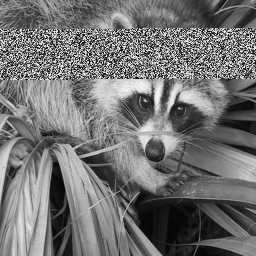
\includegraphics[width=0.3\textwidth]{face_2.png}}
    \end{subcaptionbox}
    \hfill
    \begin{subcaptionbox}{A bitmap image with irreparable errors.}
        {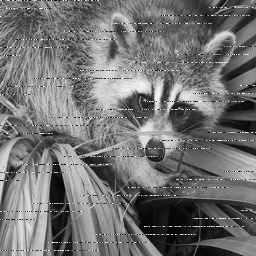
\includegraphics[width=0.3\textwidth]{face_3.png}}
    \end{subcaptionbox}
    \hfill
    \begin{subcaptionbox}{Figure A, repaired.}
        {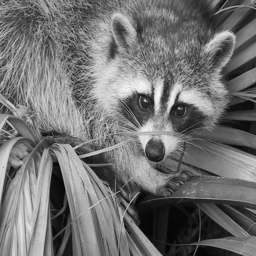
\includegraphics[width=0.3\textwidth]{face_2_repaired.png}}
    \end{subcaptionbox}
    
    \caption{Image source: \texttt{scipy.datasets.face}.}
\end{figure}


\printbibliography[heading=bibintoc]

\end{document}
